\documentclass[english,hidelinks, 11 pt, class=report,crop=false]{standalone}
\usepackage[T1]{fontenc}
%\usepackage[utf8]{inputenc}
\usepackage{lmodern} % load a font with all the characters
\usepackage{geometry}
\geometry{verbose,paperwidth=16.1 cm, paperheight=24 cm, inner=2.3cm, outer=1.8 cm, bmargin=2cm, tmargin=1.8cm}
\setlength{\parindent}{0bp}
\usepackage{import}
\usepackage[subpreambles=false]{standalone}
\usepackage{amsmath}
\usepackage{amssymb}
\usepackage{esint}
\usepackage{babel}
\usepackage{tabu}
\makeatother
\makeatletter

\usepackage{titlesec}
\usepackage{ragged2e}
\RaggedRight
\raggedbottom
\frenchspacing

\usepackage{graphicx}
\usepackage{float}
\usepackage{subfig}
\usepackage{placeins}
\usepackage{cancel}
\usepackage{framed}
\usepackage{wrapfig}
\usepackage[subfigure]{tocloft}
\usepackage[font=footnotesize,labelfont=sl]{caption} % Figure caption
\usepackage{bm}
\usepackage[dvipsnames, table]{xcolor}
\definecolor{shadecolor}{rgb}{0.105469, 0.613281, 1}
\colorlet{shadecolor}{Emerald!15} 
\usepackage{icomma}
\makeatother
\usepackage[many]{tcolorbox}
\usepackage{multicol}
\usepackage{stackengine}

\usepackage{esvect} %For vectors with capital letters

% For tabular
\usepackage{array}
\usepackage{multirow}
\usepackage{longtable} %breakable table

% Ligningsreferanser
\usepackage{mathtools} % for mathclap
%\mathtoolsset{showonlyrefs}

% sections without numbering in toc
\newcommand\tsec[1]{\phantomsection \addcontentsline{toc}{section}{#1}
	\section*{#1}}

% index
\usepackage{imakeidx}
\makeindex[title=Indeks]

%Footnote:
\usepackage[bottom, hang, flushmargin]{footmisc}
\usepackage{perpage} 
\MakePerPage{footnote}
\addtolength{\footnotesep}{2mm}
\renewcommand{\thefootnote}{\arabic{footnote}}
\renewcommand\footnoterule{\rule{\linewidth}{0.4pt}}
\renewcommand{\thempfootnote}{\arabic{mpfootnote}}

%colors
\definecolor{c1}{cmyk}{0,0.5,1,0}
\definecolor{c2}{cmyk}{1,0.25,1,0}
\definecolor{n3}{cmyk}{1,0.,1,0}
\definecolor{neg}{cmyk}{1,0.,0.,0}


\newcommand{\nreq}[1]{
\begin{equation}
	#1
\end{equation}
}


% Equation comments
\newcommand{\cm}[1]{\llap{\color{blue} #1}}


\usepackage[inline]{enumitem}
\newcounter{rg}
\numberwithin{rg}{chapter}


\newcommand{\reg}[2][]{\begin{tcolorbox}[boxrule=0.3 mm,arc=0mm,colback=blue!3] {\refstepcounter{rg}\phantomsection \large \textbf{\therg \;#1} \vspace{5 pt}}\newline #2  \end{tcolorbox}\vspace{-5pt}}
\newcommand{\regdef}[2][]{\begin{tcolorbox}[boxrule=0.3 mm,arc=0mm,colback=blue!3] {\refstepcounter{rg}\phantomsection \large \textbf{\therg \;#1} \vspace{5 pt}}\newline #2  \end{tcolorbox}\vspace{-5pt}}
\newcommand{\words}[1]{\begin{tcolorbox}[boxrule=0.3 mm,arc=0mm,colback=teal!3] #1  \end{tcolorbox}\vspace{-5pt}}

\newcommand\alg[1]{\begin{align*} #1 \end{align*}}

\newcommand\eks[2][]{\begin{tcolorbox}[boxrule=0.3 mm,arc=0mm,enhanced jigsaw,breakable,colback=green!3] {\large \textbf{\ekstitle #1} \vspace{5 pt}\\} #2 \end{tcolorbox}\vspace{-5pt} }

\newcommand{\st}[1]{\begin{tcolorbox}[boxrule=0.0 mm,arc=0mm,enhanced jigsaw,breakable,colback=yellow!12]{ #1} \end{tcolorbox}}

\newcommand{\spr}[1]{\begin{tcolorbox}[boxrule=0.3 mm,arc=0mm,enhanced jigsaw,breakable,colback=yellow!7] {\large \textbf{\sprtitle} \vspace{5 pt}\\} #1 \end{tcolorbox}\vspace{-5pt} }

\newcommand{\sym}[1]{\colorbox{blue!15}{#1}}

\newcommand{\info}[2]{\begin{tcolorbox}[boxrule=0.3 mm,arc=0mm,enhanced jigsaw,breakable,colback=cyan!6] {\large \textbf{#1} \vspace{5 pt}\\} #2 \end{tcolorbox}\vspace{-5pt} }

\newcommand\algv[1]{\vspace{-11 pt}\begin{align*} #1 \end{align*}}

\newcommand{\regv}{\vspace{5pt}}
\newcommand{\mer}{\textsl{\note}: }
\newcommand{\mers}[1]{{\footnotesize \mer #1}}
\newcommand\vsk{\vspace{11pt}}
\newcommand{\tbs}{\vspace{5pt}}
\newcommand\vs{\vspace{-11pt}}
\newcommand\vsb{\vspace{-16pt}}
\newcommand\br{\\[5 pt]}
\newcommand{\figp}[1]{../fig/#1}
\newcommand\algvv[1]{\vs\vs\begin{align*} #1 \end{align*}}
\newcommand{\y}[1]{$ {#1} $}
\newcommand{\os}{\\[5 pt]}
\newcommand{\prbxl}[2]{
\parbox[l][][l]{#1\linewidth}{#2
	}}
\newcommand{\prbxr}[2]{\parbox[r][][l]{#1\linewidth}{
		\setlength{\abovedisplayskip}{5pt}
		\setlength{\belowdisplayskip}{5pt}	
		\setlength{\abovedisplayshortskip}{0pt}
		\setlength{\belowdisplayshortskip}{0pt} 
		\begin{shaded}
			\footnotesize	#2 \end{shaded}}}
\newcommand{\fgbxr}[2]{
	\parbox[r][][l]{#1\linewidth}{#2
}}		

\renewcommand{\cfttoctitlefont}{\Large\bfseries}
\setlength{\cftaftertoctitleskip}{0 pt}
\setlength{\cftbeforetoctitleskip}{0 pt}

\newcommand{\bs}{\\[3pt]}
\newcommand{\vn}{\\[6pt]}
\newcommand{\fig}[1]{\begin{figure}[H]
		\centering
		\includegraphics[]{\figp{#1}}
\end{figure}}

\newcommand{\figc}[2]{\begin{figure}
		\centering
		\includegraphics[]{\figp{#1}}
		\caption{#2}
\end{figure}}
\newcommand{\arc}[1]{{
		\setbox9=\hbox{#1}%
		\ooalign{\resizebox{\wd9}{\height}{\texttoptiebar{\phantom{A}}}\cr\textit{#1}}}}

\newcommand{\sectionbreak}{\clearpage} % New page on each section

\newcommand{\nn}[1]{
\begin{equation*}
	#1
\end{equation*}
}

\newcommand{\enh}[1]{\,\textrm{#1}}

%asin, atan, acos
\DeclareMathOperator{\atan}{atan}
\DeclareMathOperator{\acos}{acos}
\DeclareMathOperator{\asin}{asin}

% Comments % old cm, ggb cm is new
%\newcommand{\cm}[1]{\llap{\color{blue} #1}}

%%%

\newcommand\fork[2]{\begin{tcolorbox}[boxrule=0.3 mm,arc=0mm,enhanced jigsaw,breakable,colback=yellow!7] {\large \textbf{#1 (\expl)} \vspace{5 pt}\\} #2 \end{tcolorbox}\vspace{-5pt} }
 
%colors
\newcommand{\colr}[1]{{\color{red} #1}}
\newcommand{\colb}[1]{{\color{blue} #1}}
\newcommand{\colo}[1]{{\color{orange} #1}}
\newcommand{\colc}[1]{{\color{cyan} #1}}
\definecolor{projectgreen}{cmyk}{100,0,100,0}
\newcommand{\colg}[1]{{\color{projectgreen} #1}}

% Methods
\newcommand{\metode}[2]{
	\textsl{#1} \\[-8pt]
	\rule{#2}{0.75pt}
}

%Opg
\newcommand{\abc}[1]{
	\begin{enumerate}[label=\alph*),leftmargin=18pt]
		#1
	\end{enumerate}
}
\newcommand{\abcs}[2]{
	\begin{enumerate}[label=\alph*),start=#1,leftmargin=18pt]
		#2
	\end{enumerate}
}
\newcommand{\abcn}[1]{
	\begin{enumerate}[label=\arabic*),leftmargin=18pt]
		#1
	\end{enumerate}
}
\newcommand{\abch}[1]{
	\hspace{-2pt}	\begin{enumerate*}[label=\alph*), itemjoin=\hspace{1cm}]
		#1
	\end{enumerate*}
}
\newcommand{\abchs}[2]{
	\hspace{-2pt}	\begin{enumerate*}[label=\alph*), itemjoin=\hspace{1cm}, start=#1]
		#2
	\end{enumerate*}
}

% Exercises


\newcounter{opg}
\numberwithin{opg}{section}

\newcounter{grub}
\numberwithin{opg}{section}
\newcommand{\op}[1]{\vspace{15pt} \refstepcounter{opg}\large \textbf{\color{blue}\theopg} \vspace{2 pt} \label{#1} \\}
\newcommand{\eksop}[2]{\vspace{15pt} \refstepcounter{opg}\large \textbf{\color{blue}\theopg} (#1) \vspace{2 pt} \label{#2} \\}

\newcommand{\nes}{\stepcounter{section}
	\setcounter{opg}{0}}
\newcommand{\opr}[1]{\vspace{3pt}\textbf{\ref{#1}}}
\newcommand{\oeks}[1]{\begin{tcolorbox}[boxrule=0.3 mm,arc=0mm,colback=white]
		\textit{\ekstitle: } #1	  
\end{tcolorbox}}
\newcommand\opgeks[2][]{\begin{tcolorbox}[boxrule=0.1 mm,arc=0mm,enhanced jigsaw,breakable,colback=white] {\footnotesize \textbf{\ekstitle #1} \\} \footnotesize #2 \end{tcolorbox}\vspace{-5pt} }


% tag exercises
\newcommand{\tagop}[1]{ 
{\small \color{Gray} #1} \os
}

% License
\newcommand{\lic}{
This book is part of the \net{https://sindrsh.github.io/openmathbooks/}{OpenMathBooks} project. OpenMathBooks © 2022 by Sindre Sogge Heggen is licensed under CC BY-NC-SA 4.0. To view a copy of this license, visit \net{http://creativecommons.org/licenses/by-nc-sa/4.0/}{http://creativecommons.org/licenses/by-nc-sa/4.0/}}

%referances
\newcommand{\net}[2]{{\color{blue}\href{#1}{#2}}}
\newcommand{\hrs}[2]{\hyperref[#1]{\color{blue}#2 \ref*{#1}}}
\newcommand{\refunnbr}[2]{\hyperref[#1]{\color{blue}#2}}


\newcommand{\openmath}{\net{https://sindrsh.github.io/openmathbooks/}{OpenMathBooks}}
\newcommand{\am}{\net{https://sindrsh.github.io/FirstPrinciplesOfMath/}{AM1}}
\newcommand{\mb}{\net{https://sindrsh.github.io/FirstPrinciplesOfMath/}{MB}}
\newcommand{\tmen}{\net{https://sindrsh.github.io/FirstPrinciplesOfMath/}{TM1}}
\newcommand{\tmto}{\net{https://sindrsh.github.io/FirstPrinciplesOfMath/}{TM2}}
\newcommand{\amto}{\net{https://sindrsh.github.io/FirstPrinciplesOfMath/}{AM2}}
\newcommand{\eksbm}{
\footnotesize
Dette er opppgaver som har blitt gitt ved sentralt utformet eksamen i Norge. Oppgavene er laget av Utdanningsdirektoratet. Forkortelser i parantes viser til følgende:
\begin{center}
	\begin{tabular}{c|c}
		E & Eksempeloppgave \\
		V/H & Eksamen fra vårsemesteret/høstsemesteret\\
		G/1P/1T/R1/R2 & Fag  \\
		XX & År 20XX \\
		D1/D2 & Del 1/Del 2
	\end{tabular}
\end{center}
Tekst og innhold kan her være noe endret i forhold til originalen.
}

%Excel og GGB:

\newcommand{\g}[1]{\begin{center} {\tt #1} \end{center}}
\newcommand{\gv}[1]{\begin{center} \vspace{-11 pt} {\tt #1}  \end{center}}
\newcommand{\cmds}[2]{{\tt #1}\\
	#2}

% outline word
\newcommand{\outl}[1]{{\boldmath \color{teal}\textbf{#1}}}
%line to seperate examples
\newcommand{\linje}{\rule{\linewidth}{1pt} }


%Vedlegg
\newcounter{vedl}
\newcounter{vedleq}
\renewcommand\thevedl{\Alph{vedl}}	
\newcommand{\nreqvd}{\refstepcounter{vedleq}\tag{\thevedl \thevedleq}}

%%% Writing code

\usepackage{listings}


\definecolor{codegreen}{rgb}{0,0.6,0}
\definecolor{codegray}{rgb}{0.5,0.5,0.5}
\definecolor{codepurple}{rgb}{0.58,0,0.82}
\definecolor{backcolour}{rgb}{0.95,0.95,0.92}

\newcommand{\pymet}[1]{{\ttfamily\color{magenta} #1}}
\newcommand{\pytype}[1]{{\ttfamily\color{codepurple} #1}}

\lstdefinestyle{mystyle}{
	backgroundcolor=\color{backcolour},   
	commentstyle=\color{codegreen},
	keywordstyle=\color{magenta},
	numberstyle=\tiny\color{codegray},
	stringstyle=\color{codepurple},
	basicstyle=\ttfamily\footnotesize,
	breakatwhitespace=false,         
	breaklines=true,                 
	captionpos=b,                    
	keepspaces=true,                 
	numbers=left,                    
	numbersep=5pt,                  
	showspaces=false,                
	showstringspaces=false,
	showtabs=false,                  
	tabsize=2,
	inputencoding=utf8,
	extendedchars=true,
	literate= {
		{å}{{\aa}}1 
		{æ}{{\ae}}1 
		{ø}{{\o}}1
	}
}

\lstset{style=mystyle}

\newcommand{\python}[1]{
\begin{tcolorbox}[boxrule=0.3 mm,arc=0mm,colback=white]
\lstinputlisting[language=Python]{#1}
\end{tcolorbox}}
\newcommand{\pythonut}[2]{
\begin{tcolorbox}[boxrule=0.3 mm,arc=0mm,colback=white]
\small 
%\textbf{Kode}
\lstinputlisting[language=Python]{#1}	
\vspace{11pt}
\textbf{Utdata} \\ \ttfamily
#2
\end{tcolorbox}}
%%%

%page number
%\usepackage{fancyhdr}
%\pagestyle{fancy}
%\fancyhf{}
%\renewcommand{\headrule}{}
%\fancyhead[RO, LE]{\thepage}

\usepackage{datetime2}
%%\usepackage{sansmathfonts} for dyslexia-friendly math
\usepackage[]{hyperref}


% note
\newcommand{\note}{Note}
\newcommand{\notesm}[1]{{\footnotesize \textsl{\note:} #1}}
\newcommand{\selos}{See the solutions manual.}

\newcommand{\texandasy}{The text is written in \LaTeX\ and the figures are made with the aid of Asymptote.}

\newcommand{\rknut}{Calculate.}
\newcommand\sv{\vsk \textbf{Answer} \vspace{4 pt}\\}
\newcommand{\ekstitle}{Example }
\newcommand{\sprtitle}{The language box}
\newcommand{\expl}{explanation}

% answers
\newcommand{\mulansw}{\notesm{Multiple possible answers.}}	
\newcommand{\faskap}{Chapter}

% exercises
\newcommand{\opgt}{\newpage \phantomsection \addcontentsline{toc}{section}{Exercises} \section*{Exercises for Chapter \thechapter}\vs \setcounter{section}{1}}

\newcommand{\grubop}[1]{\vspace{15pt} \refstepcounter{grub}\large \textbf{\color{blue} Ponder \thegrub} \vspace{2 pt} \label{#1} \\}
\newcommand{\grubr}[1]{\vspace{3pt}\textbf{Ponder \ref{#1}}}


% references
\newcommand{\reftab}[1]{\hrs{#1}{Table}}
\newcommand{\rref}[1]{\hrs{#1}{Rule}}
\newcommand{\dref}[1]{\hrs{#1}{Definition}}
\newcommand{\refkap}[1]{\hrs{#1}{Chapter}}
\newcommand{\refsec}[1]{\hrs{#1}{Section}}
\newcommand{\refdsec}[1]{\hrs{#1}{Subsection}}
\newcommand{\refved}[1]{\hrs{#1}{Appendix}}
\newcommand{\eksref}[1]{\textsl{#1}}
\newcommand\fref[2][]{\hyperref[#2]{\textsl{Figure \ref*{#2}#1}}}
\newcommand{\refop}[1]{{\color{blue}Exercise \ref{#1}}}
\newcommand{\refops}[1]{{\color{blue}Exercise \ref{#1}}}

%%% SECTION HEADLINES %%%

% Our numbers
\newcommand{\likteikn}{The equal sign}
\newcommand{\talsifverd}{Numbers, digits and values}
\newcommand{\koordsys}{Coordinate systems}

% Calculations
\newcommand{\adi}{Addition}
\newcommand{\sub}{Subtraction}
\newcommand{\gong}{Multiplication}
\newcommand{\del}{Division}

%Factorization and order of operations
\newcommand{\fak}{Factorization}
\newcommand{\rrek}{Order of operations}

%Fractions
\newcommand{\brgrpr}{Introduction}
\newcommand{\brvu}{Values, expanding and simplifying}
\newcommand{\bradsub}{Addition and subtraction}
\newcommand{\brgngheil}{Fractions multiplied by integers}
\newcommand{\brdelheil}{Fractions divided by integers}
\newcommand{\brgngbr}{Fractions multiplied by fractions}
\newcommand{\brkans}{Cancelation of fractions}
\newcommand{\brdelmbr}{Division by fractions}
\newcommand{\Rasjtal}{Rational numbers}

%Negative numbers
\newcommand{\negintro}{Introduction}
\newcommand{\negrekn}{The elementary operations}
\newcommand{\negmeng}{Negative numbers as amounts}

%Calculation methods
\newcommand{\delmedtihundre}{Deling med 10, 100, 1\,000 osv.}

% Geometry 1
\newcommand{\omgr}{Terms}
\newcommand{\eignsk}{Attributes of triangles and quadrilaterals}
\newcommand{\omkr}{Perimeter}
\newcommand{\area}{Area}

%Algebra 
\newcommand{\algintro}{Introduction}
\newcommand{\pot}{Powers}
\newcommand{\irrasj}{Irrational numbers}

%Equations
\newcommand{\ligintro}{Introduction}
\newcommand{\liglos}{Solving with the elementary operations}
\newcommand{\ligloso}{Solving with elementary operations summarized}

%Functions
\newcommand{\fintro}{Introduction}
\newcommand{\lingraf}{Linear functions and graphs}

%Geometry 2
\newcommand{\geoform}{Formulas of area and perimeter}
\newcommand{\kongogsim}{Congruent and similar triangles}
\newcommand{\geofork}{Explanations}

% Names of rules
\newcommand{\adkom}{Addition is commutative}
\newcommand{\gangkom}{Multiplication is commutative}
\newcommand{\brdef}{Fractions as rewriting of division}
\newcommand{\brtbr}{Fractions multiplied by fractions}
\newcommand{\delmbr}{Fractions divided by fractions}
\newcommand{\gangpar}{Distributive law}
\newcommand{\gangparsam}{Paranthesis multiplied together}
\newcommand{\gangmnegto}{Multiplication by negative numbers I}
\newcommand{\gangmnegtre}{Multiplication by negative numbers II}
\newcommand{\konsttre}{Unique construction of triangles}
\newcommand{\kongtre}{Congruent triangles}
\newcommand{\topv}{Vertical angles}
\newcommand{\trisum}{The sum of angles in a triangle}
\newcommand{\firsum}{The sum of angles in a quadrilateral}
\newcommand{\potgang}{Multiplication by powers}
\newcommand{\potdivpot}{Division by powers}
\newcommand{\potanull}{The special case of \boldmath $a^0$}
\newcommand{\potneg}{Powers with negative exponents}
\newcommand{\potbr}{Fractions as base}
\newcommand{\faktgr}{Factors as base}
\newcommand{\potsomgrunn}{Powers as base}
\newcommand{\arsirk}{The area of a circle}
\newcommand{\artrap}{The area of a trapezoid}
\newcommand{\arpar}{The area of a parallelogram}
\newcommand{\pyt}{Pythagoras's theorem}
\newcommand{\forform}{Ratios in similar triangles}
\newcommand{\vilkform}{Terms of similar triangles}
\newcommand{\omkrsirk}{The perimeter of a circle (and the value of $ \bm \pi $)}
\newcommand{\artri}{The area of a triangle}
\newcommand{\arrekt}{The area of a rectangle}
\newcommand{\liknflyt}{Moving terms across the equal sign}
\newcommand{\funklin}{Linear functions}



\begin{document}
\newpage
\section{Indexes}
\subsection{Introduction}
\parbox{0.6\linewidth}{
In economy, an \outl{index} is the value of a ratio indicating the change of a quantity. For example, the Norwegian ice cream ''kroneis'' cost 0.75\enh{kr} when it was released in 1953, while in 2021 it cost 27\enh{kr}. Then the ratio of the price in 2021 to the price in 1953 is
	\[ \frac{\text{price in 2021}}{\text{price in 1953}}=\frac{27}{0.75}= 36 \]
}
\parbox[r]{0.3\linewidth}{
\includegraphics[scale=2]{kr}}\\[2pt]
In this conjuncture 36 is the index of the price change of ''kroneis'' between 1953 and 2021.

\begin{comment}
	\regv 
	\reg[Indeks]{\vsb
	\[ \frac{\text{verdi 1}}{\text{verdi 2}}\cdot 100 = \text{indeks} \]
	}
	\eks[1]{
	En vare kostet 15\,kr i 2017 og 5\,kr i 1990. Regn ut indeksen for prisendringen fra 2017 til 1990.
	
	\sv 
	Vi deler prisen fra 2017 med prisen fra 1990 og ganger medd 100:
	\[ \frac{15}{5}\cdot 100 = 300 \]
	Indeksen er altså 300.
	}
	\eks[2]{
	En vare kostet i 2000 10 kr. In
	}
\end{comment}
\subsection{Consumer price index and base year}
The \outl{Consumer price index} (CPI) is an index indicating a comparative price level of urban merchandise and services, such as\vs

\parbox[t]{0.49\linewidth}{\begin{itemize}
		\item Food and non-alcoholic beverages
		\item Alcoholic beverages and tobacco
		\item Clothing and footwear
		\item Housing, water, electricity, gas and other fuels
		\item Furnishings, household equipment and routine maintenance

\end{itemize}}
\parbox[t]{0.49\linewidth}{\begin{itemize}
		\item Health	
		\item Transport
		\item Communications
		\item Recreation and culture
		\item Education
		\item Restaurants and hotels

\end{itemize}}
To compare something a reference is needed, and the consumer price index use the price level of the aforementioned wares and servise in 2015 as a reference. Hence, 2015 is called the \outl{base year}\footnote{The year set as the base year changes with time. Before 2015 became the base year, 1998 was.}, with it's index set to 100.\regv
\reg[Base year]{The index of a base year equals 100. 2015 is the base year of the consumer price index.}\vsk

The below table presents the CPI for the  years 2011\,-\,2020
\begin{center}
	\begin{tabular}{c|c}
		År &  KPI \\ \hline
		2020 & 112,2\\
		2019 & 	110,8\\
		2018 &  112,2 \\
		2017&	105,5\\
		2016&	103,6\\
		2015&	100\\
		2014&	97,9\\
		2013&	95,9\\
		2012&	93,9\\
		2011&	93,3\\
	\end{tabular}
	\captionof{table}{Consumer price index for the years 2011-2021. Numbers from \net{https://www.ssb.no/en/priser-og-prisindekser/konsumpriser/statistikk/konsumprisindeksen}{SSB}. \label{KPI}}
\end{center}
According to the table, we can, for example, read the following:
\begin{itemize}
	\item Since CPI in 2017 was 105.5, the prices have increased by 5.5\% since 2015.
	\item Since CPI in 2011 was 93.3, the prices were 7,7\% lower in 2011 than in 2015.
\end{itemize}
\reg[Percentage change relative to the base year]{\vs \vs
\[ \text{index}-100=\text{percentage change relative to the base year} \]
}
\eks[1]{
In july 2021 CPI for food was 109,4. How much have the price for food changed compared to the base year?

\sv $ {109.4-100=9.4}  $. The price of food has increased by 9,4\% compared to the base year.
}
\newpage
\eks[2]{
In july 2021 CPI for footwear was 98.0. How much have the price for footwear changed compared to the base year?

\sv 
$ {98,0-100=-2} $. Hence, the price of footwear is reduced by 2\% compared to the base year.  
}
\subsection{Kroneverdi}
As mentioned, a ''kroneis'' cost 0.75\enh{kr} in 1953, and 27\enh{kr} in 2021. When at two distinct points of time we have to pay a \textsl{different} price for the \textsl{same} merchandise it will often mean that the\footnote{Here, 'krone' can be substituted by any currency.} \outl{krone value} has changed;\textsl{ 1\enh{kr} in 1957 was more worth than 1\enh{kr} i 2021.
}\vsk

The krone value for a given year is defined as 100 divided by the CPI of that year: \regv
	
\reg[Kroneverdi \label{kroneverdi}]{\vs
\[ \text{kroneverdi}=\frac{100}{\text{KPI}} \]
{\footnotesize\mer Kroneverdien for basisåret (2015) er 1.}
}
\eks[1]{
CPI in 2012 was 93.9. Calculate the krone value in 2012.

\sv \vs
\algv{
\text{krone value in 2012} &= \frac{100}{93.9}\\
&\approx 1.06
}
This means that 1\enh{kr} in 2012 was equivalent to 1,06\enh{kr} in the base year.
}
\newpage
\reg[Real value \label{realverdi}]{
The real value of an amount of money yields the value of these money in the base year.	
\[ \text{real value} = \text{original value}\cdot \text{currency value} \]
}
\eks{
	In 1928, the CPI was 3.2, and in 2020, the CPI was 112.2. Which had the greater real value, 10,000 NOK in 1928 or 350,000 NOK in 2020?
	
	\sv
	We have that
	\begin{align*}
		\text{Krone value in 1928} &= \frac{100}{3.2}
	\end{align*}
	Thus,
	\begin{align*}
		\small
		\text{The value of 10,000 NOK from 1928 in base year} &= 10,000 \text{ NOK} \cdot \frac{100}{3.2} \\
		&= 312,500 \text{ NOK}
	\end{align*}
	Furthermore,
	\begin{align*}
		\text{Krone value in 2020} &= \frac{100}{112.2}
	\end{align*}
	Thus,
	\begin{align*}
		\footnotesize
		\text{The value of 350,000 NOK from 1928 in base year} &= 350,000 \text{ NOK} \cdot \frac{100}{112.2} \\
		&\approx 311,943 \text{ NOK}
	\end{align*}
	Therefore, 10,000 NOK was worth more in 1928 than what 350,000 NOK was worth in 2020.
}

\subsection{Real Wages and Nominal Wages}
How well off we are depends on how much we earn and what the price level is. Suppose you had an annual salary of 500,000 NOK in both 2020 and 2019. \hyperref[KPI]{\textsl{Table \ref*{KPI}}} then tells us that you had better purchasing power in 2019 because the price level (CPI) was lower than in 2020. \vspace{5pt}

An increase in the price level is the same as a decrease in the value of the currency. This means that if your salary was the same in 2019 and 2020, the \textsl{real value} of your salary is higher in 2019 than in 2020. The original salary and the real value of the salary are so commonly used in statistics that they have their own names:\vspace{5pt}

\reg[Real Wages and Nominal Wages\label{realnomonn}]{
	Nominal wages are the wages received in a given year. \vspace{5pt}
	
	Real wages are the real value of the nominal wages.
}

\eks{
	In 2016, Per earned 450,000 NOK, while in 2012, he earned 420,000 NOK. In 2016, the CPI was 103.6, while in 2012, it was 93.9. In which of these years did Per have better purchasing power?
	
	\sv
	To find out in which year Per had better purchasing power, we check which year had the highest real wage\footnote{We obtain the CPI values from \hyperref[KPI]{\textsl{Table 1}} for this calculation.} (see \rref{realverdi}):
	\begin{align*}
		\text{Real wage in 2016} &= 450,000 \cdot \frac{100}{103.6} \text{ NOK} \\
		&\approx 434,363 \text{ NOK} \\
		\text{Real wage in 2012} &= 420,000 \cdot \frac{100}{93.9} \text{ NOK} \\
		&\approx 447,284 \text{ NOK}
	\end{align*}
	Per's real wage was highest in 2012; therefore, he had better purchasing power in that year.
}
\newpage

\reg[Value Following an Index]{
	A value is said to have \textit{followed an index} if the value and index at two points in time are equal.
	\[ \frac{\text{value at time 1}}{\text{index at time 1}} = \frac{\text{value at time 2}}{\text{index at time 2}} \]
}

\eks[1]{
	The table below shows an overview of prices recorded in a store for two items at two different points in time.
	\begin{center}
		\begin{tabular}{r|r|r|}
			& \textbf{2010} & \textbf{2020}	\\ \hline
			chocolate & 11.00 NOK & 13.40 NOK \\
			soda & 12.50 NOK & 19.00 NOK
		\end{tabular}
	\end{center}
	In 2010, the CPI was 92.1, and in 2020, the CPI was 112.1. Has the price of any of the items followed the index?
	
	\sv
	
	We have that
	\begin{align*}
		\frac{\text{price of chocolate in 2010}}{\text{CPI in 2010}} &\approx \frac{11.00}{92.1} \approx 0.119 \\
		\frac{\text{price of chocolate in 2020}}{\text{CPI in 2020}} &\approx \frac{13.40}{112.1} \approx 0.119
	\end{align*}
	Furthermore,
	\begin{align*}
		\frac{\text{price of soda in 2010}}{\text{CPI in 2010}} &\approx \frac{12.50}{92.1} \approx 0.136 \\
		\frac{text{price of soda in 2020}}{\text{CPI in 2020}} &\approx \frac{19.00}{112.1} \approx 0.169
	\end{align*}
	So, it's reasonable to say that the price of chocolate has followed the index, while the price of soda has not.
}

\section{Loans and Savings}
\subsection{Loans}
Sometimes we don't have enough money to buy what we want and, therefore, need to take out a loan from a bank. The bank then lends us a certain \textit{loan amount} in exchange for us paying it back, along with \textit{interest}, over a specified period. Typically, we pay the bank what is called the \textit{installment amount} along the way, which consists of \textit{principal} and interest. The amount we owe the bank at any given time is called \textit{debt}. \vspace{5pt}

Suppose a bank lends us 100,000 NOK, which is the loan amount. The loan is to be repaid over 5 years, with one installment amount each year, and the interest rate is 10%. There are different ways to repay a loan, but the following generally applies:
\begin{itemize}
	\item \textbf{The sum of all installments should equal the loan amount}.\vspace{5pt}
	
	To simplify our example, we decide to repay the loan with equal installments each year. Since 100,000 NOK should be distributed equally over 5 years, the annual installment should be $ \frac{100,000}{5} \text{ NOK} = 20,000 \text{ NOK} $.
	\item \textbf{What is paid in installments should be deducted from the debt}.\vspace{5pt}
	
	The initial debt is 100,000 NOK, but in the first year, we pay 20,000 NOK in installments, so the debt becomes $ 100,000 \text{ NOK} - 20,000 \text{ NOK} = 80,000 \text{ NOK} $. In the second year, we pay another 20,000 NOK, making the debt $ 80,000 \text{ NOK} - 20,000 \text{ NOK} = 60,000 \text{ NOK} $, and so on for the next three years.
	\item \textbf{Interest should be calculated on the debt}.\vspace{5pt}
	
	Since the debt in the first year is 100,000 NOK, we must pay $ 100,000 \text{ NOK} \times 0.1 = 10,000 \text{ NOK} $ in interest. In the second year, with a debt of 80,000 NOK, we must pay $ 80,000 \text{ NOK} \times 0.1 = 8,000 \text{ NOK} $ in interest, and so on for the next three years.
	\item \textbf{The installment amount is the sum of the principal and interest}.\vspace{5pt}
	
	From the first and third points, we deduce that:
	\begin{center}
		\begin{tabular}{c|c|c}
			& 1st year & 2nd year \\ \hline
			Installment amount & $\begin{matrix} 20,000 \text{ NOK} + 10,000 \text{ NOK} \\ = \\ 30,000 \text{ NOK} \end{matrix} $ & $\begin{matrix} 20,000 \text{ NOK} + 8,000 \text{ NOK} \\ = \\ 28,000 \text{ NOK} \end{matrix} $
		\end{tabular}
	\end{center}
	And so on for the next three years.
	\item \textbf{The loan is complete when the debt is zero, and all interest is paid}.\vspace{5pt}
	
	If we have paid installments of 20,000 NOK for 5 years, the debt is reduced to zero. If we have also paid all the interest, the loan is complete.\vspace{5pt}
	
	{\footnotesize\textit{Note: You always have the right to pay larger installments than originally agreed upon. If you pay off the entire debt, provided that any interest has also been paid, the loan will be terminated.}}
\end{itemize}
\vspace{5pt}
\textbf{Amortizing Loans and Annuity Loans}\vspace{5pt}

Two common types of loans are \textit{amortizing loans} and \textit{annuity loans}. The loan from the example we just saw is an amortizing loan because the installments are of equal size. If the installment amounts had been equal, it would have been an annuity loan instead. If the loan amount, interest rate, and repayment period are the same, an amortizing loan will always result in lower overall expenses. However, for individuals, annuity loans are very popular because it is easier to plan finances when paying the same amount each time. \vspace{5pt}

\textbf{Credit Cards}\vspace{5pt}\\
\prbxl{0.6}{Credit cards are a payment card that works in such a way that if you, for example, use the card to pay 10,000 NOK, you are borrowing the money from the bank. After a period agreed upon with the bank, it will charge interest on your debt. When you pay this debt }\qquad
\parbox{0.3\linewidth}{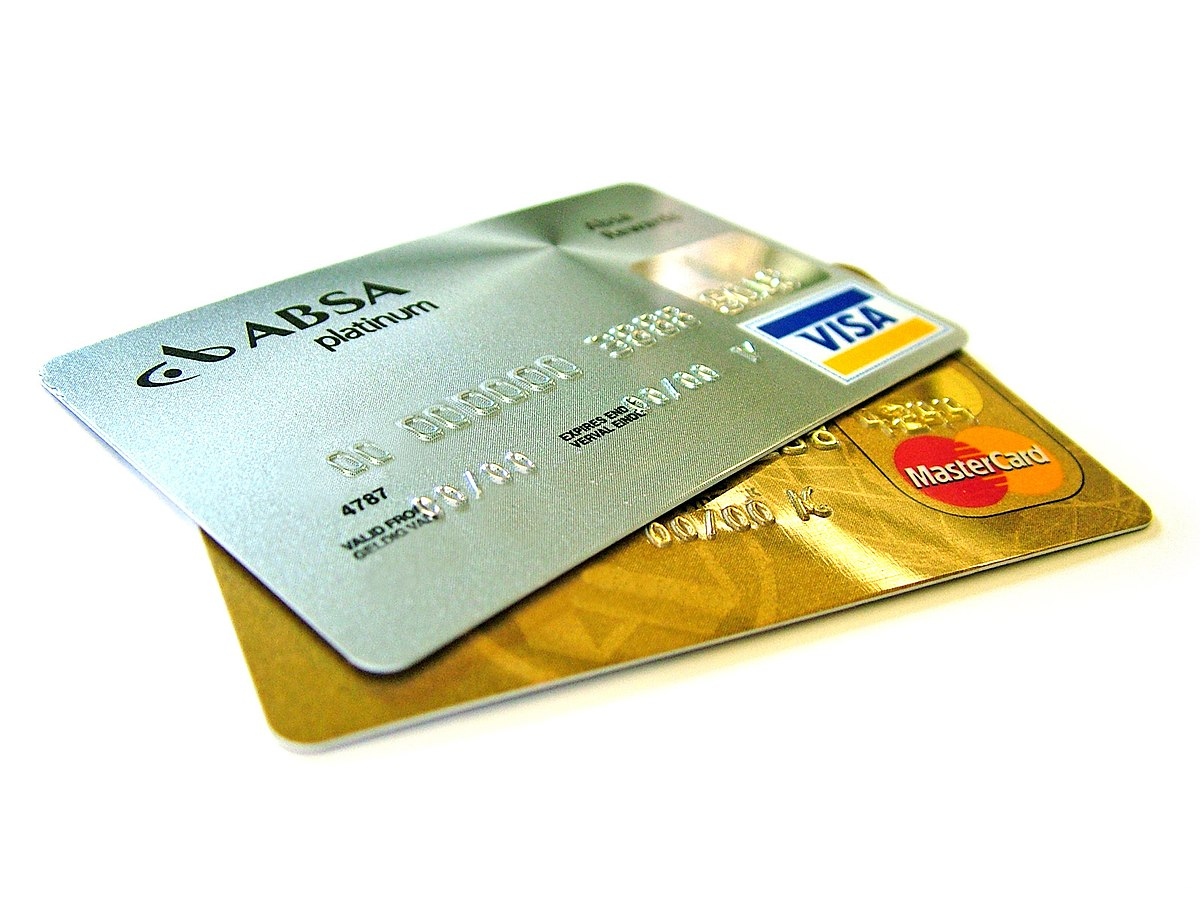
\includegraphics[scale=0.1]{kred}}\\[2pt]
is partly up to you, but generally, credit cards have very high-interest rates, so it is wise to pay it off before the interest starts accruing!

\regv
\reg[Loans]{
	\small
	\renewcommand{\arraystretch}{1.5}
	\begin{tabular}{>{\bfseries}r l}
		loan amount & The amount we borrow from the bank. \\
		debt & What we owe the bank at any given time. \\
		interest & Percentage of debt to be paid.\\
		principal & What we pay down on the debt.  \\
		& The sum of the principal equals the loan amount.\\
		& New debt $ = $ old debt $ - $ principal \\
		interest & debt $ \cdot $ interest \\
		installment & principal $ + $ interest \\
		amortizing loan & A loan where the installments are of equal size. \\
		annuity loan & A loan where the installment amounts are equal. \\
		credit card & A payment card that creates a loan from the bank.
	\end{tabular}
}
\newpage
\eks[1]{
	From a bank, you borrow 300,000 NOK with a 3% annual interest rate. The loan is to be repaid as an amortizing loan with 5 annual installment amounts.\vspace{5pt}
	\textbf{a)} What is the annual principal payment?\vspace{5pt}
	\textbf{b)} What is your debt after paying the third installment amount?\vspace{5pt}
	\textbf{c)} How much do you have to pay in interest for the fourth installment amount?\vspace{5pt}
	\textbf{d)} What is the amount of the fourth installment?\vspace{5pt}
	
	\textbf{Solution:}\vspace{5pt}
	
	\textbf{a)} Since 300,000 NOK is to be paid over 5 years, the annual principal payment is
	\[ \frac{300,000 \text{ NOK}}{5} = 60,000 \text{ NOK} \]
	
	\textbf{b)} When the third installment is paid, you have paid three installments. That means your debt is
	\[ 300,000 - 60,000 \cdot 3 = 300,000 - 180,000 = 120,000 \text{ NOK} \]
	So, 120,000 NOK.
	
	\textbf{c)} From the answer to part b), we know that the debt is 180,000 NOK when the fourth installment is to be paid. 3% of the debt is then
	\[ 180,000 \cdot 0.03 = 5,400 \text{ NOK} \]
	So, 5,400 NOK.
	
	\textbf{d)} The installment amount is equal to the principal plus interest. Based on the answers to parts a) and c), we know that the fourth installment amount is
	\[ 60,000 \text{ NOK} + 5,400 \text{ NOK} = 65,400 \text{ NOK} \]
	So, the fourth installment amount is 65,400 NOK.
}

\eks[2]{
	From a bank, you borrow 100,000 NOK with a 6.4\% annual interest rate. The loan is to be repaid as an annuity loan over 5 years, and the bank has calculated that the installment amount will be 24,000 NOK.\vspace{5pt}
	
	Calculate the principal and interest for the first installment amount.
	
	\sv
	
	In the first year, the debt is 100,000 NOK, and you must pay 6.4% of this in interest:
	\[ 100,000 \cdot 0.064 = 6,400 \text{ NOK} \]
	So, you must pay 6,400 NOK in interest in the first year.\vspace{5pt}
	
	We have that
	\[ \text{installment amount} = \text{principal} + \text{interest} \]
	So, the principal is
	\[ \text{principal} = \text{installment amount} - \text{interest} = 24,000 \text{ NOK} - 6,400 \text{ NOK} = 17,600 \text{ NOK} \]
	So, you must pay 17,600 NOK in principal in the first year.
}

\newpage
\subsection{Savings; Deposit Interest and Expected Return}
\subsubsection{Deposit Interest}
We have seen that we must pay interest when we borrow money from a bank, but if we instead put money (make a deposit) in a bank, we \textsl{earn} interest: \regv

\reg[Deposit Interest]{
	Deposit interest is a percentage increase in the money you have in the bank, repeated over fixed time intervals (monthly, annually, etc.).
}

\eks[1]{
	You deposit 20,000 NOK in a bank that offers a 2\% annual savings interest rate. How much money do you have in the bank after 8 years?
	
	\sv
	To calculate deposit interest, we can use \rref{progrowth}. Since the interest rate is 2\%, the growth factor is 1.02. The original value is 20,000, and the number of changes (time) is 8:
	\[ 20,000 \cdot 1.02^8 \approx 23,433 \]
	So, you have approximately 23,433 NOK in the bank after 8 years of saving.
}

\subsubsection{Expected Return}
Another way to save money is to invest in a mutual fund. In this case, we talk about \textit{expected return}:\regv

\reg[Expected Return]{
	Expected return specifies an \textsl{expected} percentage increase of an investment, repeated over fixed time intervals.
}

\eks[1]{
	You invest 15,000 NOK in a mutual fund that expects a 5\% annual return. How much is the investment worth after 8 years with such a return?
	
	\sv
	For expected return, we can also use \rref{progrowth}. The growth factor is 1.05, the original value is 15,000, and the number of changes (time) is 8:
	\[ 15,000 \cdot 1.05^8 \approx 22,162 \]
	After 8 years, it is expected that the investment is worth 22,162 NOK.
}
\vsk

\info{Saving with Deposit Interest or Mutual Funds?}{
	Usually, the expected return on a mutual fund is higher than the deposit interest you get in a bank, but the downside is that expected return does not provide any guarantees. Expected return only indicates the increase experts anticipate. If you're lucky, the increase will be higher; if you're unlucky, it will be lower and may even result in a \textsl{reduction} of your investment. In the worst case, although extremely rare, your entire investment may end up being worth 0 NOK. \vsk
	
	Deposit interest rates can also change somewhat over time, but they can never lead to a reduction in your investment.
}

\begin{comment}
	\eks[2]{Du betaler 27\,000\,kr med et kreddittkort som krever 1,4\% rente for hver måned du betaler for seint.\os
	
	\textbf{a)} Hvor mye har du i gjeld to år etter for sein betaling?\os
	\textbf{b)} Hva er den årlige renten ved for sein betaling?
	
	\sv
	\textbf{a)} Siden renten er 1,4\%, er vekstfaktoren 1,014. Siden renten er månedlig må vi måle tiden i måneder, og to år er $ {2\cdot12=24} $ måneder. Siden starverdien er 27\,000, får vi:
	\[ 27\,000\cdot1,014^8\approx 37\,649 \]
	Etter to år har du altså ca 37\,649\,kr i gjeld.\os
	
	\textbf{b)} Siden ett år er det samme som 12 måneder blir vekstfaktoren gitt ved: 
	\[ 1,014^{12} \approx1.182\]
	}
\end{comment}


\section{Taxation}
If you have an income, you usually have to pay a portion of that money to the state. This money is called \textit{tax} (and sometimes \textit{duty}). The purpose of tax is to provide the state with the means to offer services to its citizens, such as education, healthcare, and more. Today, taxes are largely calculated by computer systems, but it is your responsibility to ensure that the calculations are correct - and that's why it's important to understand how the tax system works.\vsk

\info{Note!}{In exam questions and in real life, you will quickly realize that tax systems are presented somewhat differently than in this book. This is because tax rules can change from year to year, and in this book, we have based our explanations on the tax rules of Norway in 2018. The most important thing is not to memorize these specific rules but to learn what is meant by the terms \textit{gross income, deductions, taxable income, social security contribution}, and \textit{net income}.}

\subsection{Gross Income, Deductions, and Taxable Income}
\prbxl{0.68}{Most people have to pay 23\% of what is called \textit{taxable income}, which is \textit{gross income} minus \textit{deductions}. Gross income is the salary you receive from your employer, while deductions can be various things. \textit{Personal deductions} and \textit{minimum deductions} are something all taxpayers receive. Additionally, you can }\qquad
\prbxr{0.22}{Taxable income is sometimes called \textit{taxable basis}.} \\[-16pt]

\prbxl{0.66}{receive deductions if you pay \textit{union dues} or have donated money to charitable causes.}\qquad
\prbxr{0.24}{Union dues are what you pay to be a member of a \net{https://en.wikipedia.org/wiki/Trade_union}{trade union}.}\regv

\reg[Gross Income, Deductions, and Taxable Income]{\vs
	\begin{center}
		\begin{tabular}{c r}
			\phantom{xxxxx} &gross income	\\
			$ - $ & deductions \\ \hline
			$ = $ & taxable income \\ \hline
		\end{tabular}
	\end{center}
}

\newpage
\eks{
	Magnus's gross income is 500,000 NOK. He receives a 56,000 NOK personal deduction, a 97,600 NOK minimum deduction, and he also pays 1,000 NOK for annual membership in the union \textsl{Tekna}.\os
	How much does Magnus have to pay if he is taxed at 23% of the taxable income?
	
	\sv
	We start by calculating the taxable income, which is the gross income minus the deductions:
	\begin{center}
		\begin{tabular}{c r l}
			\phantom{xxxxx}	& 500,000 & gross income	\\
			$ - $& 56,000 & personal deduction \\
			$ - $& 97,600 & minimum deduction \\
			$ - $& 1,000 & union dues \\ \hline
			$ = $ &345,400 & taxable income \\ \hline
		\end{tabular}
	\end{center}
}

\eks{
	Jonas and his grandmother, Line, both have a salary of 150,000 NOK. Jonas is 18 years old, and Line is 71 years old.\os
	\textbf{a)} How much does Jonas have to pay in social security tax?\os
	\textbf{b)} How much does Line have to pay in social security tax?
	
	\sv
	\textbf{a)} Since Jonas is between 17 and 69 years old, he has to pay 8.2% social security tax:
	\[ 150,000 \cdot 0.082 = 12,300 \]
	So, Jonas has to pay 12,300 NOK in social security tax.
	
	\textbf{b)} Since Line is over 69 years old, she has to pay 5.1% social security tax:
	\[ 150,000 \cdot 0.051 = 7,650 \]
	So, Line has to pay 7,650 NOK in social security tax.
}

\eks{
	If you earn 550,000 NOK, the calculation of progressive tax is as follows:
	
	\begin{center}
		\small
		\begin{tabular}{c|l}
			\multirow{3}{*}{Trinn 1} 
			\\[-14pt] \hline \\
			& As the entire salary is over 237,900 NOK, you must pay \\
			& tax on ${(237,900-169,000)\,NOK = 68,900\,NOK}$. \os
			& The tax for trinn 1 is then $68,900\,NOK\cdot0.014\approx 965\,NOK$. \os \hline \\
			\multirow{4}{*}{Trinn 2} 
			& Since 550,000 NOK is over 237,900 NOK but below 598,050 NOK,\\
			& you must pay tax on ${(550,000-237,900)\,NOK = 312,100\,NOK}$.  \os
			& The tax for trinn 2 is then $312,100\,NOK\cdot0.033\approx 10,299\,NOK$. \os \hline \\
			\multirow{2}{*}{Total} 
			& In total, you must pay $ {965\,NOK+10,299\,NOK=11,264\,NOK}$\\
			& in progressive tax.
		\end{tabular}
	\end{center}
}

\newpage

\newpage
\subsection{Accounting}
In a budget, you list \textsl{expected} incomes and expenses, while in an \textit{accounting} record, you list \textsl{actual} incomes and expenses. The difference between the budget and accounting is called the \textit{deviation}. For the deviation, it is common to calculate '$ {\text{accounting}-\text{budget}} $' for incomes and results, while for expenses, you calculate '$ \text{budget}-\text{accounting} $'. This is because we want positive numbers if the incomes are higher than expected, and negative numbers if the expenses are higher than expected. \regv
\eks[]{In the example from the previous subsection (\ref*{budget}), we set up a monthly budget for Lisa.
	In March, it turned out that these were her actual incomes and expenses:
	\begin{itemize}
		\item She didn't work as much as she had planned. Net pay was 3,500 NOK.\\
		\item She spent 4,200 NOK on food.
		\item She received 4,360 NOK in away-from-home grant.
		\item In birthday gifts, she received a total of 2,000 NOK.
		\item She spent about 3,600 NOK on clothing, leisure activities, etc.
	\end{itemize}
	Set up an accounting record for Lisa's month of March.
	
	\sv \vsb
	\begin{center}
		\begin{tabular}{r r r r}
			\textbf{Incomes} & Budget & Accounting & Deviation \\ \hline 
			Salary & 4,000 & 3,500 & $ \color{red} -500 $\\
			Grant & 4,360 &  4,360 & 0\\ 
			Birthday Gifts & 0 & 2,000 & 2,000\\ \hline
			\textit{Total} & 8,360 & 9,860 & 2,000\\\hline 
			& \\
			\textbf{Expenses} & \\ \hline
			Food & 4,500 & 4,200 & 300\\
			Clothing, Leisure, etc. & 1,200 & 3,600 & $ \color{red}-2,400 $\\ \hline
			\textit{Total} & 5,700 & 7,800 & 1,900\\ \hline
			& \\ \hline
			\textbf{Result}  & 2,660 & 2,060 & $ \color{red}-600 $ \\ \hline
		\end{tabular}
	\end{center}
	So, Lisa ended up with a surplus of 2,060 NOK, but 600 NOK less than expected based on the budget. 	
}

\end{document}